
\documentclass[10pt]{article}

\usepackage{graphicx,amsmath,amssymb,subfigure,enumerate,versions}
\usepackage{multicol,multirow,mdframed}
\usepackage{epstopdf}
\usepackage{pstricks,auto-pst-pdf}
\usepackage{pst-all}
\usepackage{pst-ode}
\usepackage{pst-math}
\usepackage{hyperref}
\usepackage{listings}
%\usepackage{mcode}
\lstset{language=Matlab}
\DeclareGraphicsExtensions{.png,.jpg,.pdf}

% ************ Page Margins *************
\hoffset=-1.3in
\setlength{\textwidth}{7.5in}
%%%%% MARGINS
\topmargin 0pt
\advance \topmargin by -\headheight
\advance \topmargin by -\headsep
\textheight 9.5in

% ************ Shortcuts *************
\newcommand{\Z}{\mbox{\sf Z\hspace{-1.5mm}Z}}
\newcommand{\SolutionSeparator}{ \hfill \hfill \hrule \hfill \hfill }
\newcommand{\R}{\mbox{\rm I\hspace{-0.75mm}R}}
\columnsep=0.75in
\newcommand{\vsc}{\vspace{1mm}}
\newcommand{\D}{\Delta }
\newcommand{\ifd}{f(x)~dx}
\newcommand{\dd}{\frac{dy}{dx} \,} 
\newcommand{\der}[2]{\frac{d{#1}}{d{#2}} \,}
\newcommand{\ddx}[1]{\frac{d {#1}}{dx} \,} 
\newcommand{\ddy}[1]{\frac{d {#1}}{dy} \,} 
\newcommand{\ddz}[1]{\frac{d {#1}}{dz} \,} 
\newcommand{\ddt}[1]{\frac{d {#1}}{dt} \,} 
\newcommand{\ds}{\displaystyle } 
\newcommand{\la}{\lambda } 
\newcommand{\del}{\nabla } 
\newcommand{\zx}{\frac{\partial z}{\partial x} \,}
\newcommand{\zy}{\frac{\partial z}{\partial y} \,}
\newcommand{\dx}{\frac{\partial f}{\partial x} \,}
\newcommand{\dy}{\frac{\partial f}{\partial y} \,}
\newcommand{\pp}[2]{\frac{\partial {#1}}{\partial {#2}} \,}
\newcommand{\ppx}{\frac{\partial }{\partial x} \,}
\newcommand{\ppy}{\frac{\partial }{\partial y} \,}
\renewcommand{\thesection}{\Roman{section}}
\newcommand{\vi}{\vec{i}}
\newcommand{\vj}{\vec{j}}
\newcommand{\vk}{\vec{k}}
\newcommand{\vv}{\vec{v}}
\newcommand{\lan}{\left\langle}
\newcommand{\ran}{\right\rangle}
\newcommand{\degr}{^{\circ}}

% *** Define the printed question style ***
\newcommand{\q}[1]{ {\em #1} }
% \renewcommand{\q}[1]{ {} }

\newcommand{\notice}{ \begin{center}Some problems and solutions
    selected or adapted from \\ Stewart {\em Calculus-Early
      Transcendentals} and Hughes-Hallett {\em Calculus} .\end{center}
}

% *** Overwrite, if desired, the question format
\includeversion{Question} 
\includeversion{Solution}

\newcommand{\multicolstart}{ }
\newcommand{\multicolend}{ }

\renewenvironment{Question}
{ \begin{mdframed}[nobreak=true,hidealllines=true,backgroundcolor=gray!50,innerleftmargin=5ex] }
{ \end{mdframed} }


% *** Footnoting with symbols ***
\long\def\symbolfootnote[#1]#2{\begingroup%
\def\thefootnote{\fnsymbol{footnote}}\footnote[#1]{#2}\endgroup}

\newcommand{\WeekTitleOne}{Derivatives - Foundations}
\newcommand{\WeekTitleTwo}{Derivatives - Linearization and Applications}
\newcommand{\WeekTitleThree}{Derivatives - Modeling}
\newcommand{\WeekTitleFour}{Integrals - Foundations}
\newcommand{\WeekTitleFive}{Integrals - Techniques}
\newcommand{\WeekTitleSix}{Integrals - Modeling}
\newcommand{\WeekTitleSeven}{Differential Equations - }
\newcommand{\WeekTitleEight}{Differential Equations - }
\newcommand{\WeekTitleNine}{Differential Equations - }
\newcommand{\WeekTitleTen}{Linear Algebra - }
\newcommand{\WeekTitleEleven}{Linear Algebra - }
\newcommand{\WeekTitleTwelve}{Linear Algebra - }


\usepackage{bbding} % for Checkmarkbold
\begin{document}

\newcommand{\ub}{\underbrace}

\begin{center}
\subsection*{MNTC P01 - Week \#9 - \WeekTitleNine}
\end{center}


% % ******************** PENDULUM ********************************
\subsection*{Pendulum}
\begin{enumerate}[1.]

\item 
  \begin{Question}
    \begin{minipage}[h]{0.6\linewidth}
\vspace{0pt}
Consider the motion of a frictionless pendulum.
\begin{align*}
  \mbox{Newton's Second Law: }   m  L^2 \theta'' & = T_g \\
  & = - m L g \sin(\theta)  \\
  \mbox{Solving for $\theta''$: }\theta'' & = - \frac{g}{L} \sin(\theta) 
\end{align*}

{\bf Without} simulating the actual motion of the pendulum, we can
compute the period, $T$, using the formula below:
\begin{align*}
  T = 4 \sqrt{L/g} \int_0^{\pi/2} \frac{dx}{\sqrt{1 - k^2 \sin^2 x}}
\end{align*}
where $k = \sin\left(\frac{1}{2} \theta_0\right)$ and $g$ is the
acceleration due to gravity, $9.8 $ m/s.  
    \end{minipage} \hfill
    \begin{minipage}[h]{0.25\linewidth}
     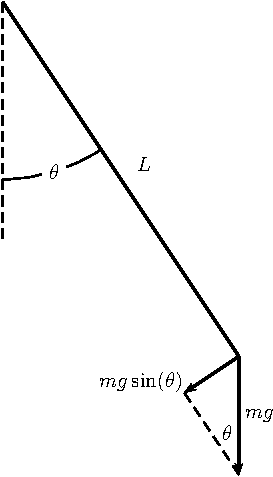
\includegraphics[width=1.0\linewidth]{graphics/Week09_Pendulum/pendulum_diagram}
    \end{minipage}

For each set of values for $L$ and $\theta_0$ given below,
\begin{enumerate}[(a)]
\item Use \verb#integral# to find the period of the pendulum oscillations,
  and
\item confirm the period by using \verb#ode45# to simulate the motion
  pendulum for exactly that length of time, and plot a graph of the
  angular {\bf velocity} against time.  The velocity should just reach
  zero at the end of one cycle.
\end{enumerate}

\begin{enumerate}[(i)]
\item $L = 2$ m, $\theta_0 = 40^o$, 
\item $L =2.5$ m, $\theta_0 = 20^o$.
\item $L =5.0$ m, $\theta_0 = 90^o$.
\end{enumerate}
  \end{Question}

\begin{Solution}

Link to the MATLAB code: \\
\href{http://www.mast.queensu.ca/~apsc171/MNTCP01/PracticeProblems/MATLAB/W09Pendulum1.m}{W09Pendulum1.m} \\
\href{http://www.mast.queensu.ca/~apsc171/MNTCP01/PracticeProblems/MATLAB/pendulumDE.m}{pendulumDE.m} \\

Note that we simply re-used the \verb#pendulumDE.m# from the lectures,
and set the friction coefficient $\mu = 0$.
  \begin{enumerate}[(i)]
  \item $L = 2$ m, $\theta_0 = 40^o$:  {\bf T = 2.9274} seconds.
  \item $L =2.5$ m, $\theta_0 = 20^o$: {\bf T = 3.1978} seconds.
  \item $L =5.0$ m, $\theta_0 = 90^o$: {\bf T = 5.2974} seconds.
  \end{enumerate}

Plots: \\
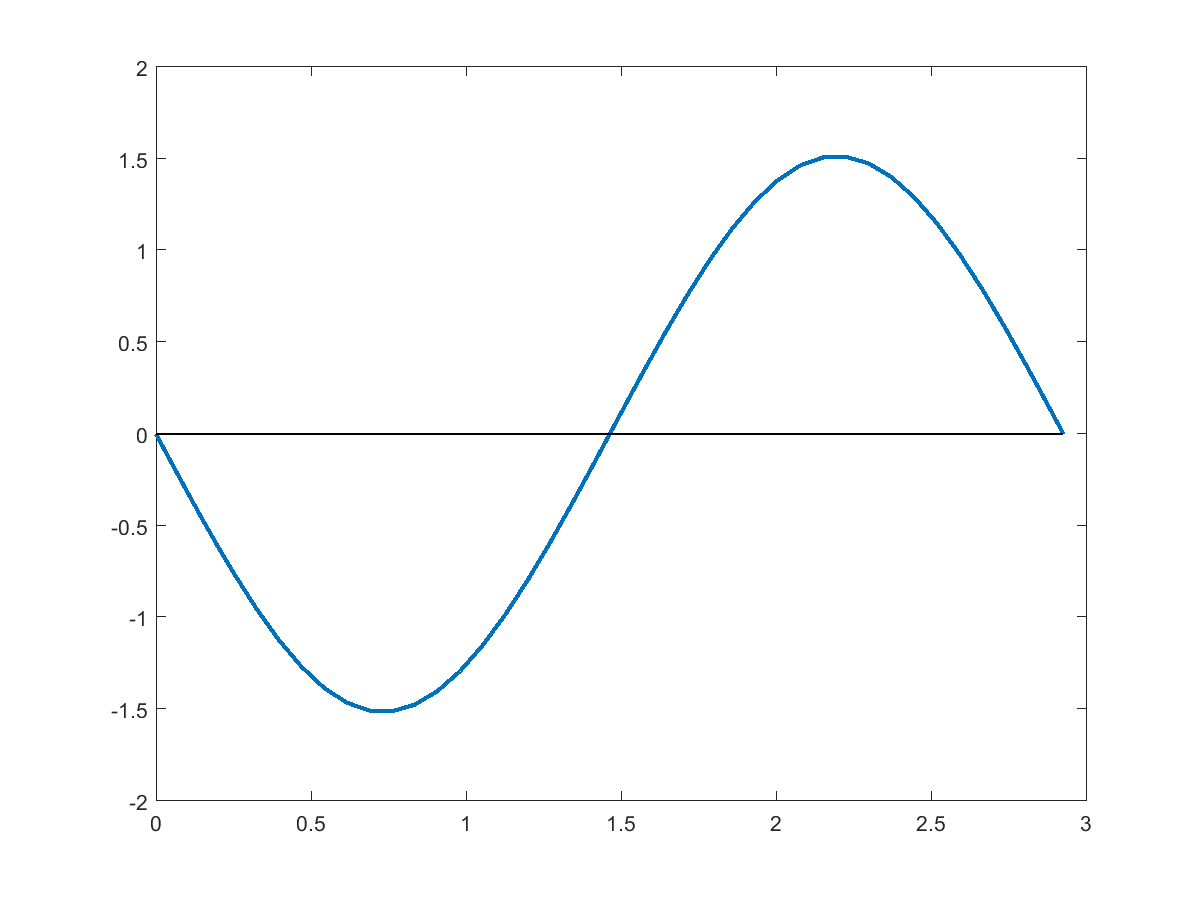
\includegraphics[width=0.33\linewidth]{graphics/Week09_Pendulum/pendulum_nofriction_1} 
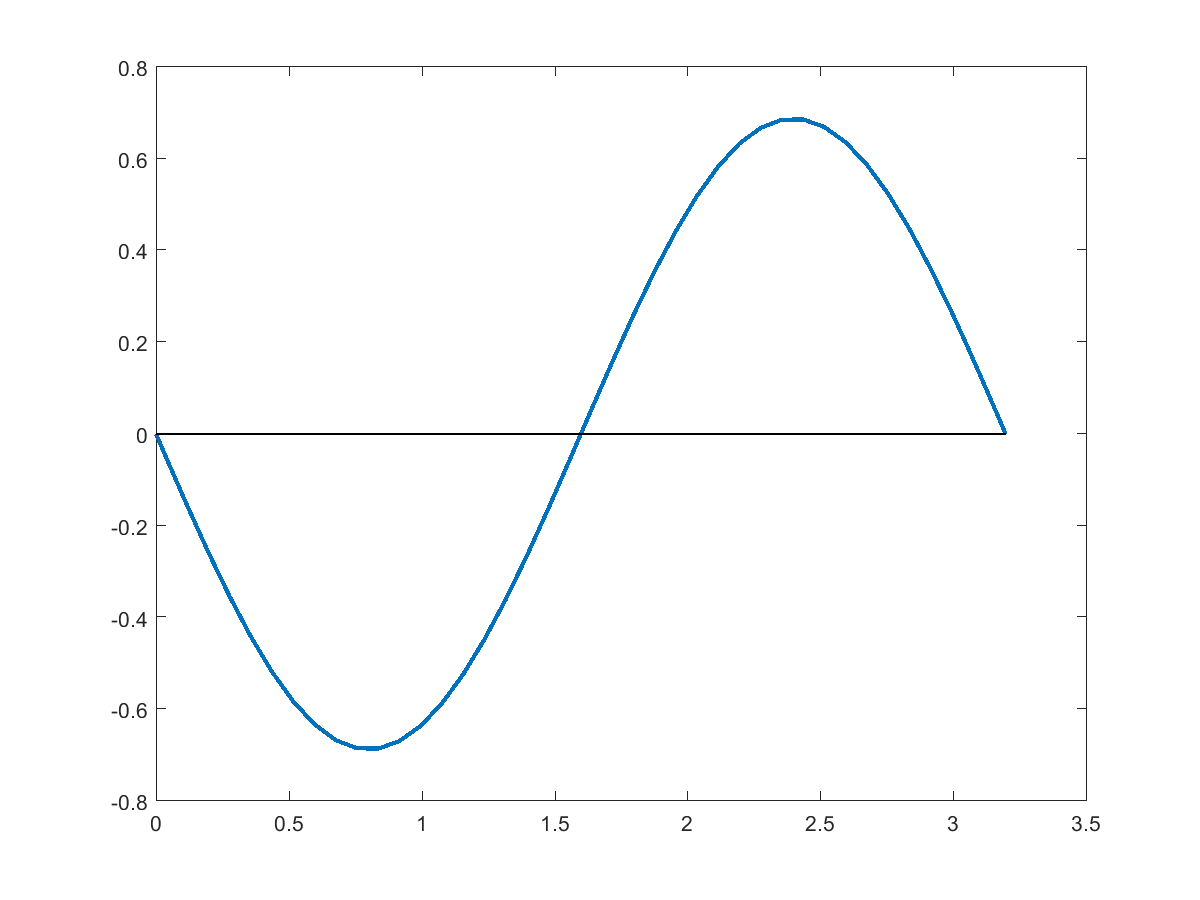
\includegraphics[width=0.33\linewidth]{graphics/Week09_Pendulum/pendulum_nofriction_2} 
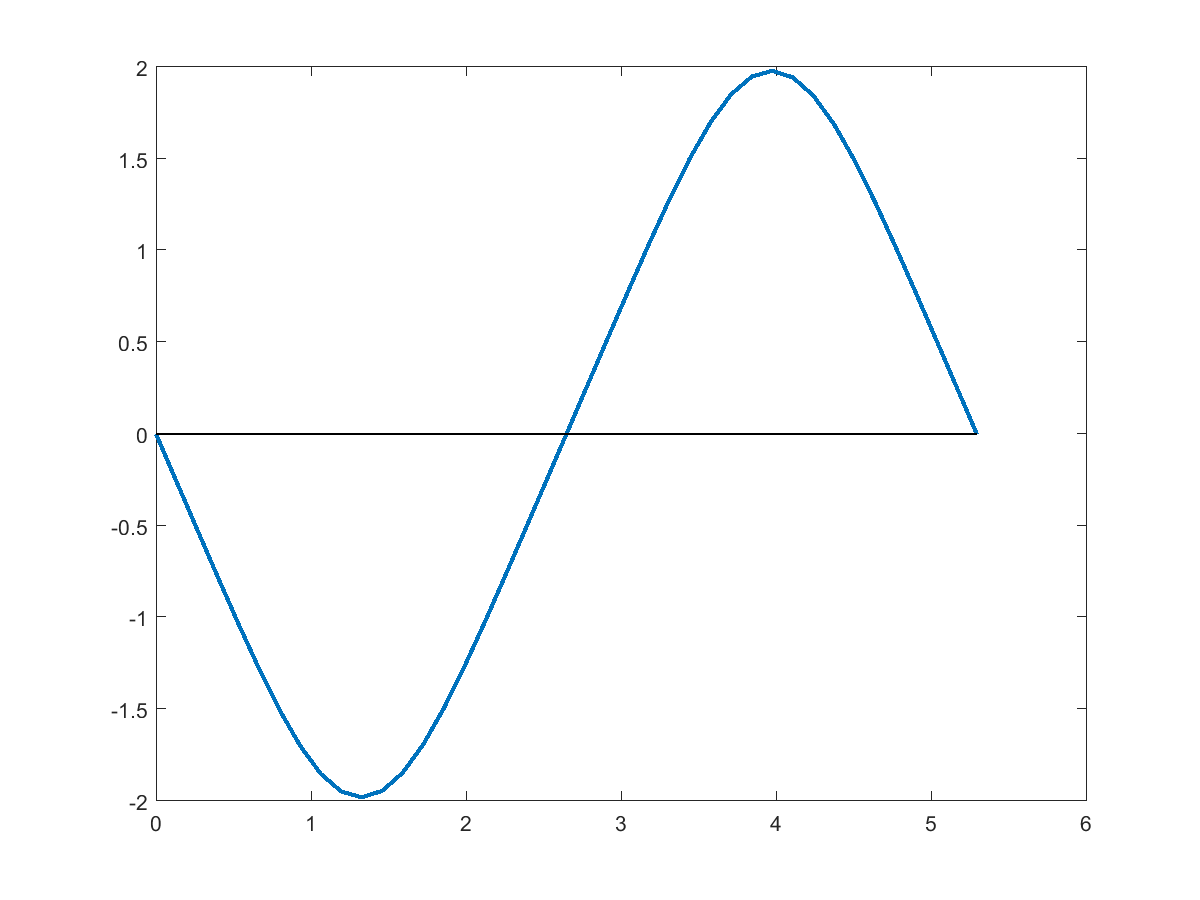
\includegraphics[width=0.33\linewidth]{graphics/Week09_Pendulum/pendulum_nofriction_3} 
\end{Solution}

%*******************************
\item
\begin{Question}
    \begin{minipage}[t]{0.7\linewidth}
\vspace{0pt}
Consider the motion of a pendulum, this time {\bf with} friction.
\begin{align*}
  \mbox{Newton's }& \mbox{ Second Law: } \\
   m  L^2 \theta'' & = T_g + T_f  \\
  & = - m L g \sin(\theta) - (\mu L^2 m) \theta' \\[3ex]
  \mbox{Solving for $\theta''$: }\theta'' & = - \frac{g}{L} \sin(\theta) - \mu 
  \theta'
\end{align*}
\begin{enumerate}[(a)]
\item Write a MATLAB function for the differential equation, and a
  script that will simulate the scenario for $L = 1.5$ m, $g = 9.8$
  m/s$^2$, and $\mu = 0.2$.  Use an initial condition of
  $\theta_0 = \frac{7\pi}{8}$, which is close to vertical.
\item Experiment with the initial {\bf angular velocity} of the
  pendulum and find the smallest {\bf positive} initial velocity that
  will result in the pendulum passing over the top of the axis of
  rotation.  Find the value to the nearest 0.1 rad/s.  

  Have MATLAB generate a plot of the angle vs time graph for both the
  initial velocity that achieves this result, and for the initial velocity 0.1 rad/s smaller, which does {\em not} go `over the top'.
\item Repeat the analysis in part (b), but this time using a {\bf
    negative} initial velocity.
\end{enumerate}
\end{minipage} \hfill
\begin{minipage}[t]{0.25\linewidth}
\vspace{0pt}
  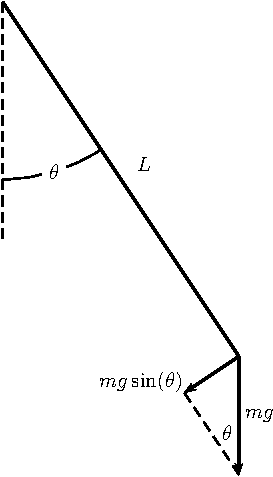
\includegraphics[width=1.0\linewidth]{graphics/Week09_Pendulum/pendulum_diagram}
\end{minipage}



\end{Question}

\begin{Solution}
Link to the MATLAB code: \\
\href{http://www.mast.queensu.ca/~apsc171/MNTCP01/PracticeProblems/MATLAB/W09Pendulum1.m}{W09Pendulum2.m} \\
\href{http://www.mast.queensu.ca/~apsc171/MNTCP01/PracticeProblems/MATLAB/pendulumDE.m}{pendulumDE.m} \\

\begin{enumerate}[(a)]
\item Here is the graph of the angle over time for the pendulum, when it has no initial velocity.

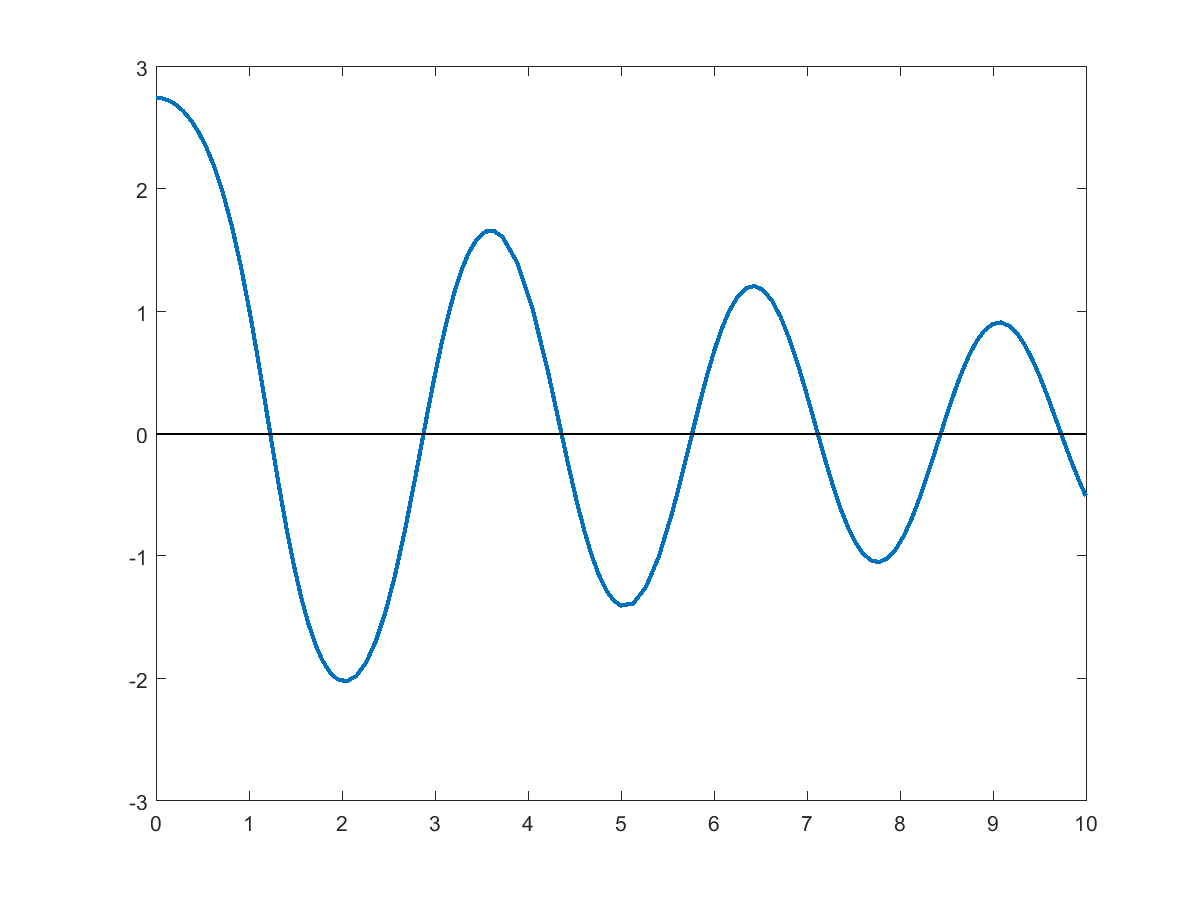
\includegraphics[width=0.33\linewidth]{graphics/Week09_Pendulum/pendulum_overtop_1} 

\item With some experimentation, we find that an initial angular
  velocity of $\theta'(0) = 1.1$ rad/s will be enough to push the
  pendulum over the top of the axis. Comparing $\theta'(0) = 1.1$ and
  1.0, we obtain the following graph of angle against time.

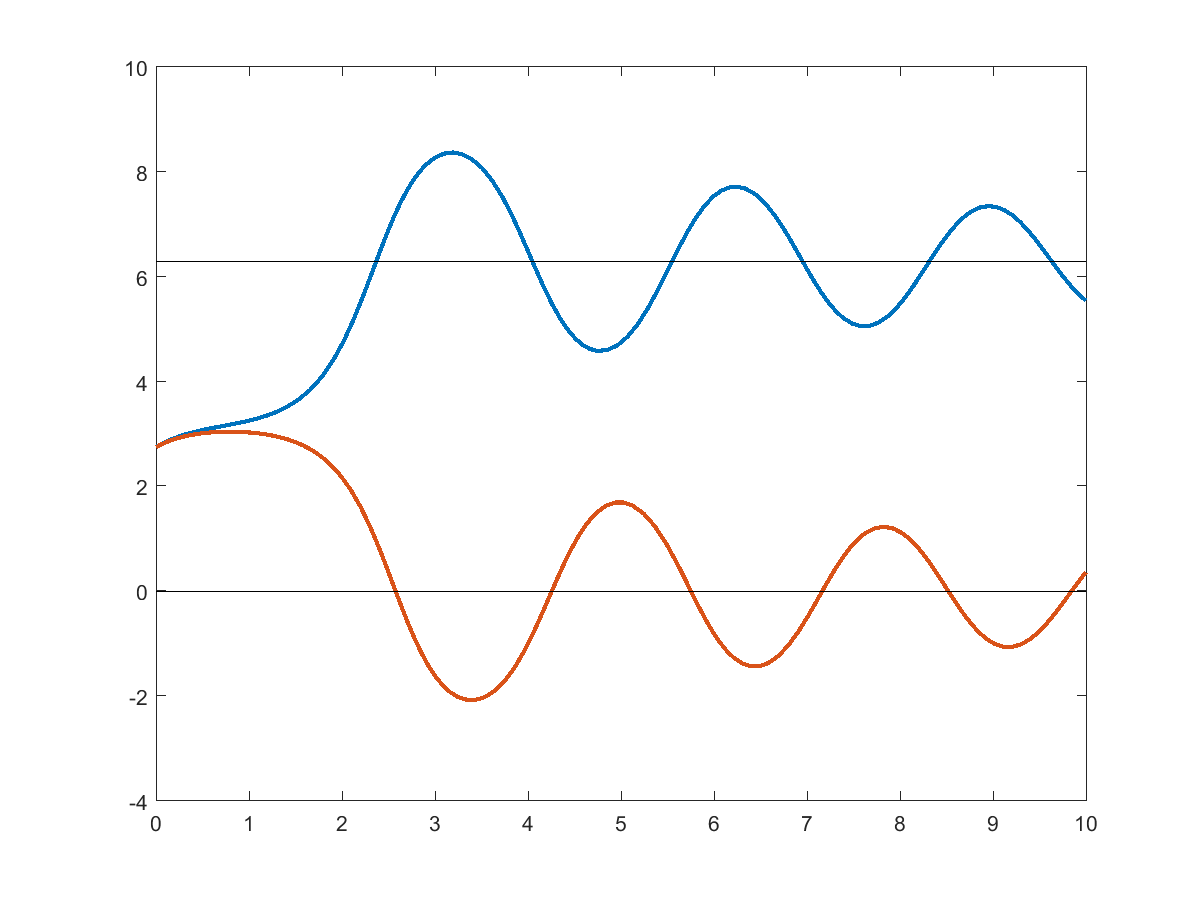
\includegraphics[width=0.5\linewidth]{graphics/Week09_Pendulum/pendulum_overtop_2} 

\item With further experimentation, we find that using negative
  initial angular velocities requires a higher initial velocity
  compared to positive initial velocities, because friction eats away
  at the effect of that first push when we are going down first and
  then over the top.  Still, a value of $\theta'(0) = -3.3$ rad/s will
  be enough to push the pendulum over the top of the axis. Comparing
  $\theta'(0) = -3.3$ and -3.2, we obtain the following graph of angle
  against time.

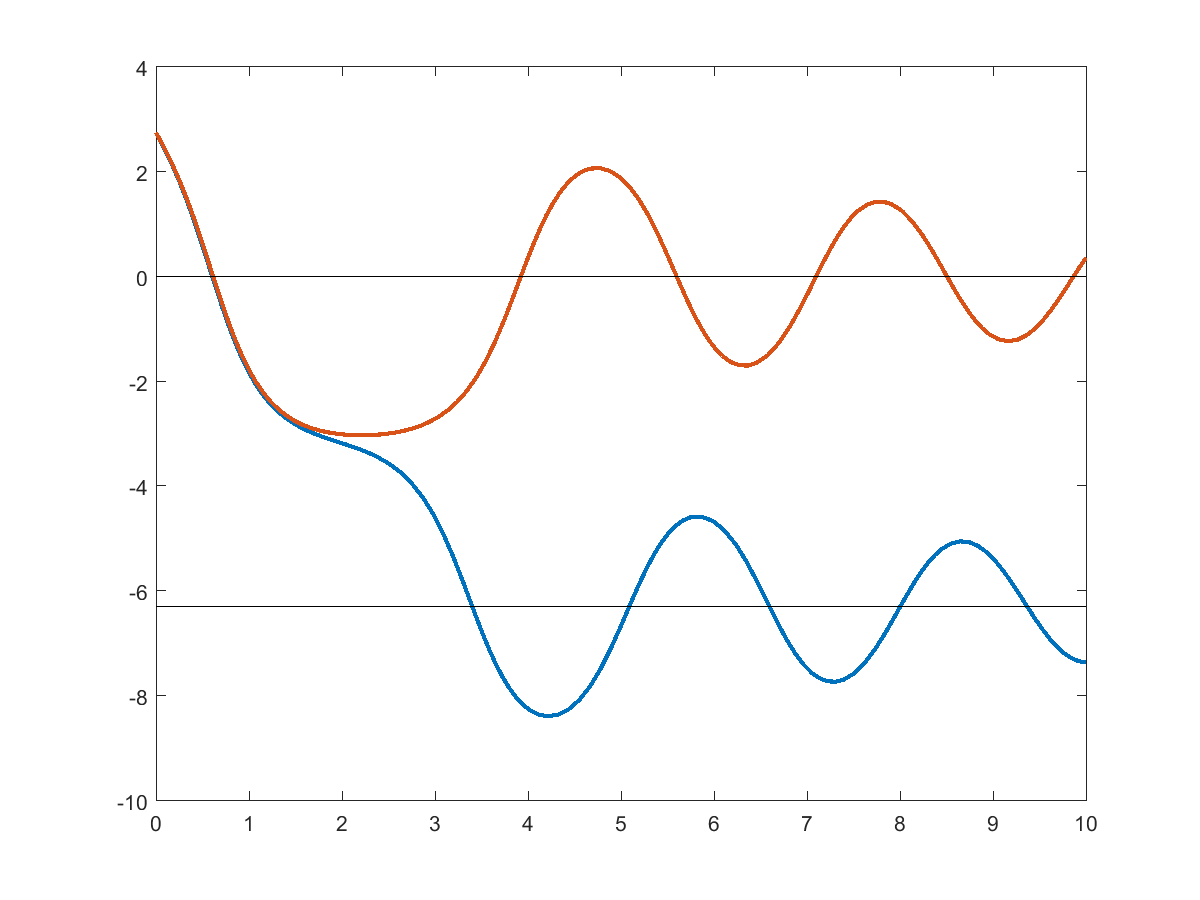
\includegraphics[width=0.5\linewidth]{graphics/Week09_Pendulum/pendulum_overtop_3} 
\end{enumerate}

\end{Solution}


\subsection*{Single Tank Problems}

%********************
\item 
\begin{Question}
  An aquarium pool has volume $2 \times 10^6$ liters.  The pool
  initially contains pure fresh water. At $t=0$ minutes, water
  containing 10 grams/liter of salt is poured into the pool at a rate
  of 60 liters/minute. The salt water instantly mixes with the fresh
  water, and the excess mixture is drained out of the pool at the same
  rate (60 liters/minute).

   \begin{enumerate}[(a)]

   \item Write a differential equation for $S(t)$, the mass of
     salt in the pool at time $t$.

   \item Use MATLAB solve the differential equation to predict $S(t)$
     over time.

   \item Based on the graph of the solution, what happens to $S(t)$ as
     $t \to \infty$?  

   \item Find this same value using only the information about the
     volume and the concentration of the incoming salt solution.

   \end{enumerate}


\end{Question}

\begin{Solution}
\begin{enumerate}
\item 
\begin{align*}
  \text{Rate of change of salt amount (g/min)} & = \text{ Rate in } - \text{ Rate out }  \\
  \text{Rate in (g/min)} & = \text{Flow rate $\times$ Concentration} \\
  & = (60 \text{ liters/min}) \times (10 \text{ g/liter}) = 600 \text{ g/min} \\
  \text{Rate out (g/min)} & = \text{Flow rate $\times$ Concentration}  \\
  & =\text{Flow rate $\times$ amount (g) / Pool volume (liters)} \\
  & = (60 \text{ liters/min}) (S(t) \text{ grams}) / (2 \times 10^6 \text{ liters}) \\
  & = (3 \times 10^{-5}) S(t) \\
  \text{Finally, we get our DE: } ~~~~~ \ddt{S} &= 600 - (3 \times 10^{-5}) S \\
\end{align*}

\item Note: to see anything interesting in this simulation, you have
  to simulate for a {\bf long} simulation time, i.e. a long
  \verb#tspan#.  Here are two graphs of the simulation results, one
  with 1000 minutes, and one with 1 million minutes.

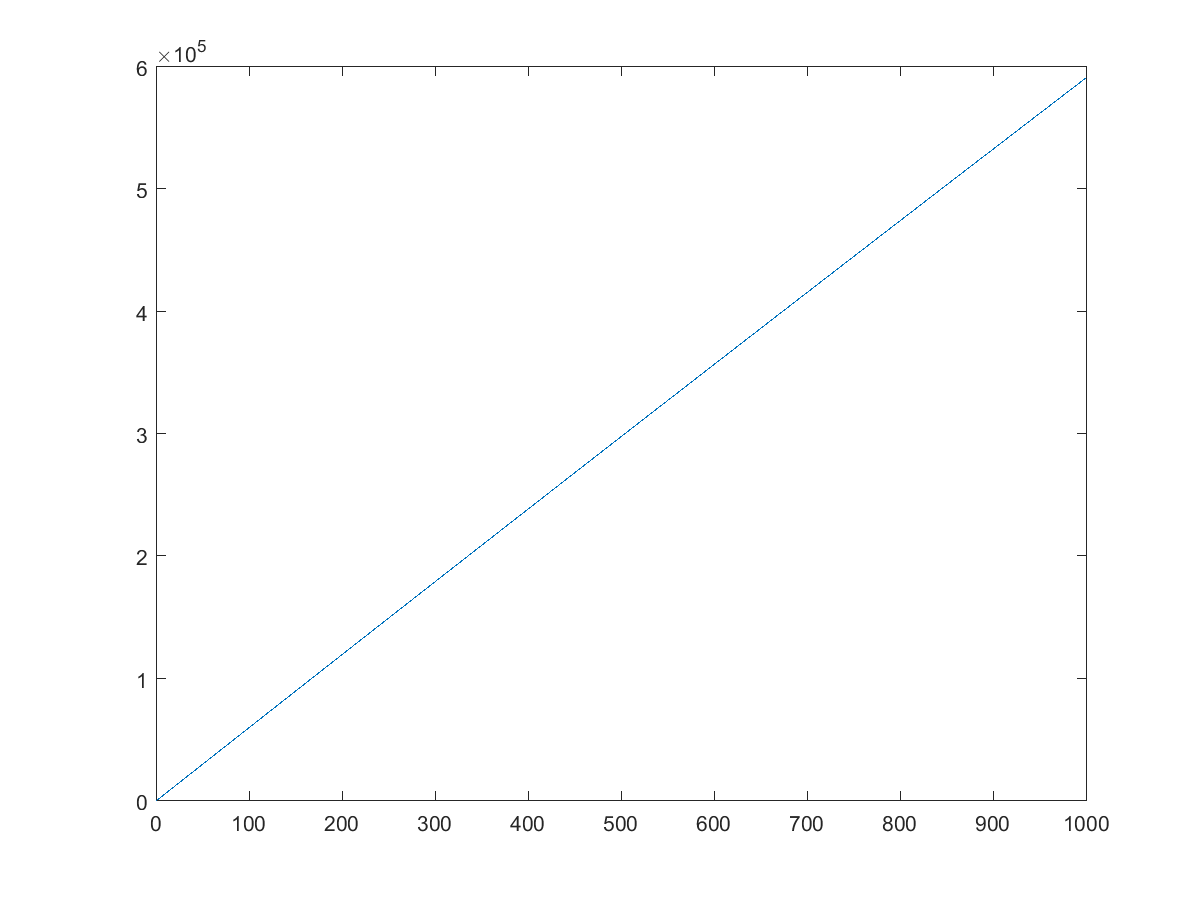
\includegraphics[width=0.45\linewidth]{graphics/Week09_Pendulum/single_tank_1a} \hfill
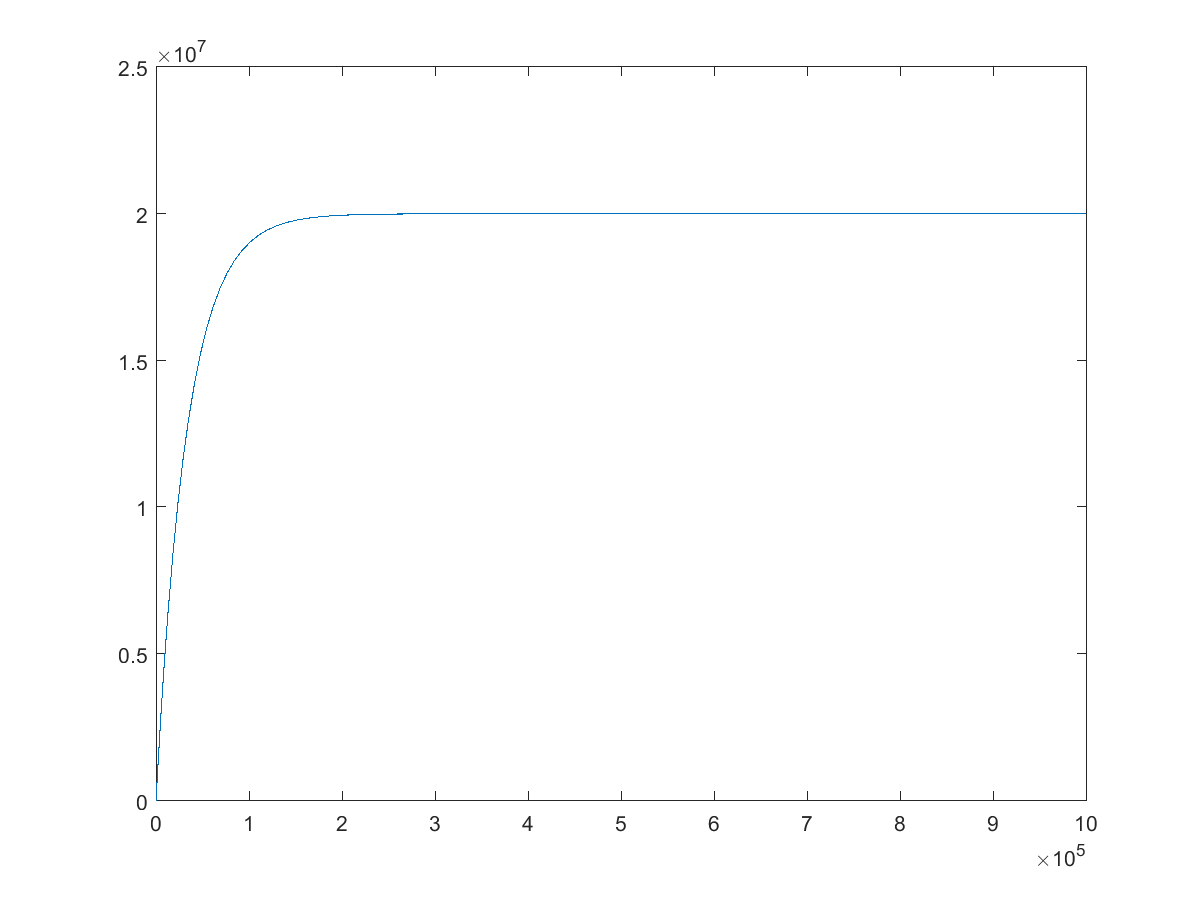
\includegraphics[width=0.45\linewidth]{graphics/Week09_Pendulum/single_tank_1b} 

\item As $t \to \infty$, we see the graph of $S(t)$ plateau at $S \to 2 \times 10^7$ grams.

\item We expect that the salt in the aquarium will tend to the same
  {\bf concentration} as the incoming water, as all of the original
  water is replaced with the new inflow solution.  At a concentration
  of 10 g/liter, in a volume of $ 2 \times 10^6$ liters, we expect to
  see eventually $S = C\times V = (10)(2 \times 10^6) = 2 \times 10^7$
  grams of salt in the aquarium, which matches our graphical results.

\end{enumerate}
\end{Solution}



% ****************************************
\item 
\begin{Question}
  A 150 litre tank initially contains 60 litres of water with 0.5 kgs
  of salt dissolved in it.  Water enters the tank at a rate of 0.9
  litres/hr and the water entering the tank has a salt concentration
  of $\frac{1}{5}(1 + \cos (t))$ kgs/litre. 
  \begin{enumerate}[(a)]
  \item Draw a diagram of the inflow and outflow for this scenario.
  \item Build a formula for the volume of water in the tank over time.
  \item Find out how long it will be until the tank overflows.
  \item Write a differential equation that describest the rate of
    change of the {\bf amount of salt} in the tank.
  \item Use MATLAB to generate a graph of the amount of salt in the
    tank over time, up until the tank overflows.
  \item How much salt is in the tank when it overflows?
  \end{enumerate}

\end{Question}

\begin{Solution}
  \begin{enumerate}[(a)]
  \item Here is a diagram of the system.

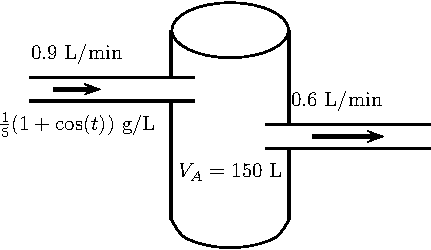
\includegraphics[width=0.45\linewidth]{graphics/Week09_SingleTanks/Tank1} 
 
  \item Since the tank has a volume of 150 L, is gaining 0.9 - 0.6 = 0.3
  L/hour, and starts at 60 L, we obtain the volume expression $V(t) = 60 + 0.3 t$.

\item Solving $V(t) = 150$ for $t$, gives us $ 60 + 0.3 t = 150$, or
  $t = 300$ hours until the tank overflows.

\item The differential equation will be the same ``rate in - rate
  out'' form.
\begin{align*}
  \text{Rate of change of salt amount (kg/hr)} & = \text{ Rate in } - \text{ Rate out } 
\end{align*}
\begin{align*}
  \text{Rate in (kg/hr)} & = \text{Flow rate $\times$ Concentration} \\
                         & = (0.9 \text{ liters/hr}) \times (\frac{1}{5} (1 + \cos(t)) \text{ kg/liter}) \\
                         & = 0.18(1 + \cos(t)) \text{kg/hr} \\
  \text{Rate out (kg/hr)} & = \text{Flow rate $\times$ Concentration}  \\
                         & =\text{Flow rate $\times$ amount (g) / Pool volume (liters)} \\
                         & = (0.6 \text{ liters/hr}) (S(t) \text{ kg}) / (60 + 0.3 t) \text{ liters}) \\
  \text{Finally, we get our DE: } ~~~~~ \ddt{S} &= 0.18 (1 + \cos(t)) - \frac{0.6}{60 + 0.3t} S
\end{align*}

\item Here is the graph of the predicted amount of salt in the tank over time. 

  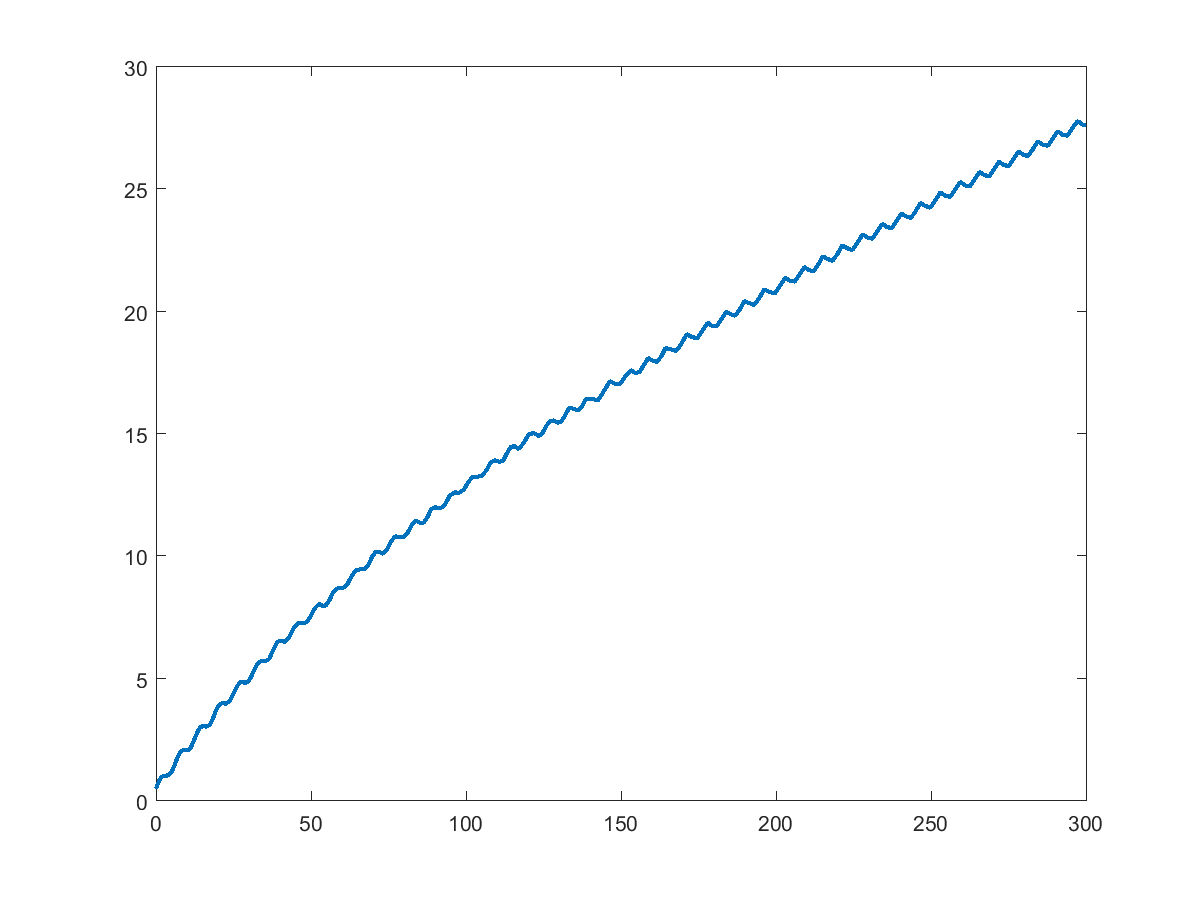
\includegraphics[width=0.75\linewidth]{graphics/Week09_SingleTanks/single_tank_2a}

  Note that the $\cos(t)$ effect has a short period ($2 \pi \approx $ 6 hours)
  relative to the 300 hours of the simulation time, which is why the
  graph looks like it has the high-frequency oscillations in it.

\item By either zooming in, or typing \verb#S# at the MATLAB command
  line to show all the \verb#S# values coming out of the simulation
  and grabbing the last one, we at the end of 300 hours that
  $S(300) \approx 27.6212$ kg of salt in the tank.

  \end{enumerate}
  
\end{Solution}

% ******************** Fish Population ********************************
\subsection*{Other First Order Models}
\item 
  \begin{Question}
    
Differential equations are not only well-suited for physics
  applications: they are are also widely used in biology, particularly
  in population models.

  Consider the fish population model below, based on a standard
  limited-resource population growth, minus a function of harvesting.

$$\frac{dP}{dt} =\underbrace{ [(10 -P)\cdot P]}_{\mbox{natural population growth rate}} -\underbrace{h(t)}_{\mbox{harvesting rate}}$$
where
\begin{itemize}
\item $P$  = population of fish (in thousands), and 
\item $\frac{dP}{dt}$  = rate of population change, in thousands per 
year
\item $h(t)$ is the harvesting rate (in thousands of fish per 
year)
\end{itemize}

We want to study the impact of two harvesting models:
\begin{itemize}
\item $h_1 = k_1$; constant harvesting
\item $h_2(t) = k_2 (\sin(\pi t) + 1)$; seasonal model where the
  harvesting has a yearly cycle.
\end{itemize}
\begin{enumerate}[(a)]

\item Generate a prediction of the population over time, starting at
  initial populations of $P(0) = 15$ for each model.  Use $k_1 = k_2 =
  5$. Produce a graph showing the predicted population over time on
  the same graph, over a long enough time interval to show the
  long-term behaviour of both solutions.

\vspace{0.2in}

One question that arises in such harvesting models is which fishing
strategy permits a higher average harvesting rate can be maintained:
seasonal harvesting, or constant harvesting?  To decide this, we note
that the average harvest rate for $h_1$ is $k_1$, and for $h_2$ is
$k_2$, so whichever value of $k_1$ and $k_2$ is larger indicates the
strategy with the greater average harvesting rate.

We will define the {\em maximum sustainable harvest rate} for both
models as the {\em highest harvest rate for which the population is
  not driven to zero.}

\item Find and report the maximum sustainable harvest level $k_1$ for
  the constant harvesting model (to the nearest integer).  (Use trial
  and error if necessary, though more insightful DE-related ways are
  possible.)  Indicate how you found the cut-off level. 

  {\em NOTE: during this process, your model will predict a population
    of zero, which will then lead to large negative populations.  This
    clearly makes no sense, so limit your plots with the command
    \verb#ylim([0, P0])#.  This same problem will also trigger
    warnings in ode45 about error tolerances; you can safely ignore
    those warnings.}

\item Generate a plot showing the population over time, using the same
  initial value used earlier, but using both the $k_1$ value just
  above, and just below the extinction level. (One line should remain
  positive, while the other should crash to zero at some point on the
  graph.)

\item Use trial and error (theory isn't much help here) to find the
  maximum sustainable harvest level $k_2$ for the cyclic harvesting
  model (to the nearest integer).  Include a plot showing the
  population over time with this harvesting level.

\item Based on your experiments, can constant harvesting or cyclic
  harvesting sustain a greater average harvest in the long run?
  Explain your reasoning.
\end{enumerate}
  \end{Question}

\begin{Solution}
\begin{enumerate}[(a)]
\item  The code in the link below generates the basic graph of the populations over time.  It can be adapted to help answer the later sections.

  Link to the MATLAB code: \\
  \href{http://www.mast.queensu.ca/~apsc171/MNTCP01/PracticeProblems/MATLAB/W09PopulationModel1.m}{W09PopulationModel1.m} \\

\includegraphics[width=3in]{graphics/Week09_PopulationModels/population_harvesting_1a}

\item Note that trial and error is just fine for this problem.  If the
  next paragraph doesn't make sense to you, feel free to skip it.  The
  important thing is to be able to do the simulations, and to generate
  the appropriate graphs.

  To get an analytic answer for the maximum sustainable harvest rate,
  we look more closely at the differential equation. We're worried
  about the population of the fish always decreasing, which would mean
  a derivative $\frac{dP}{dt}$ always being negative.  That would
  happen if the quadratic part was always smaller than $h_1 = k_1$.
  Looking at the quadratic $(10-P)P$, it will be largest at $P= 5$
  (halfway between the roots of $P=0$ and $P=10$, and will produce a
  maximum growth rate then of $(10 - 5)5 = 25$.  If we set $k_1 = 25$,
  we should just be on the threshold of sustainability.  Any value
  larger than that, and the population rate of change will always be
  negative, leading to population collapse.

  Plotting the solution for the constant harvest model at $k_1 = 25$
  and $k_1 = 26$ supports this hypothesis.
\begin{center}
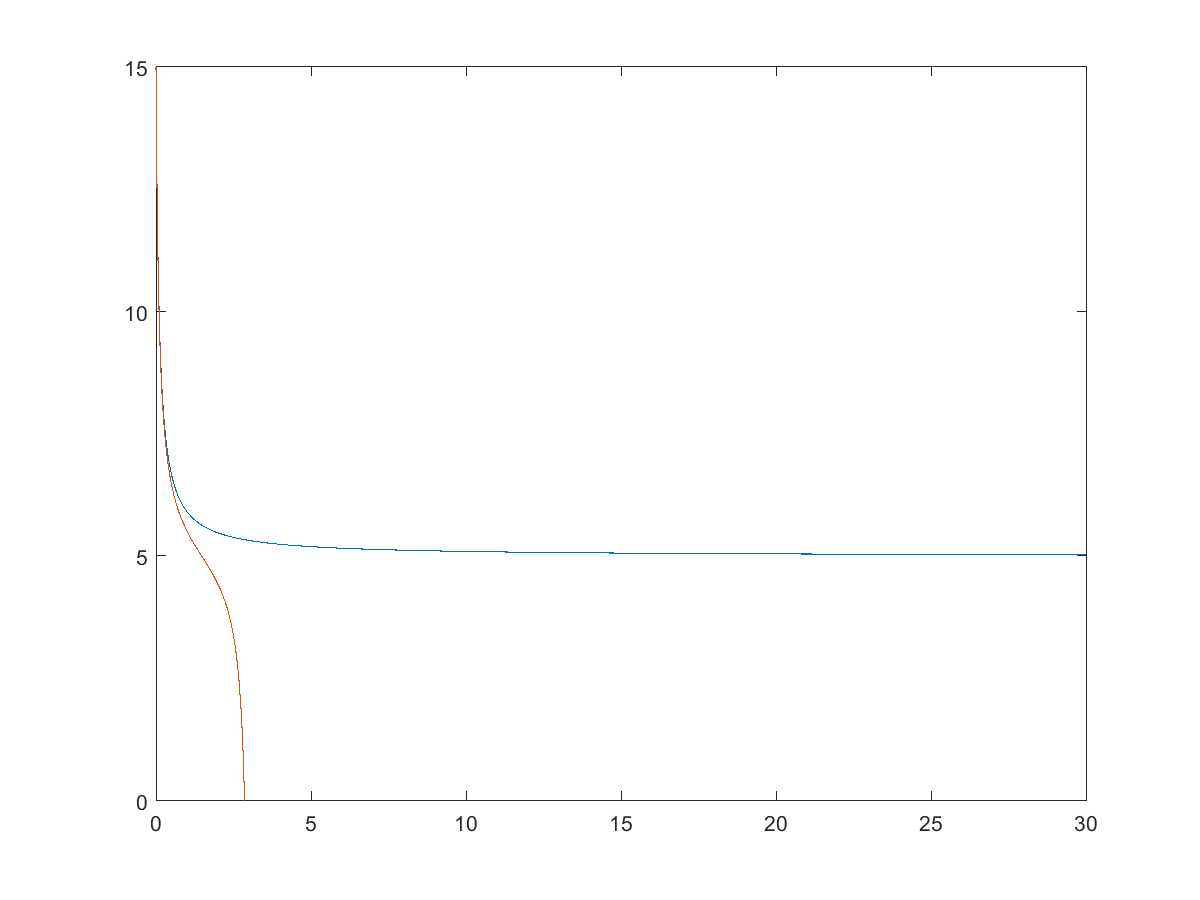
\includegraphics[width=3in]{graphics/Week09_PopulationModels/population_harvesting_1b}
\end{center}

\item In the seasonal harvest scenario, using theory to find the
  maximum sustainable value of $k_2$ isn't straightforward.  Instead,
  we simply experiment with values of $k_2$, and find that between
  $k_2 = 16$ and $k_2 = 17$, we see our seasonal pattern stop
  repeating and start reaching extinction:

\begin{center}
%\includegraphics[width=3in]{graphics/W09_PopulationModels/population_harvesting_1a}
\end{center}

\item Based on these experiments, it seems that seasonal harvesting
  leads to extinction at lower average harvesting levels, because a
  lower average rate of harvest (16 thousand fish per year) leads to
  extinction, compared to the constant harvest case (where 25 thousand
  fish per year can be harvested).
\end{enumerate}
\end{Solution}

% ********************** Tank Systems ****************
\item \begin{Question}
Consider two interconnected tanks.  Tank A initially contains $100 \; \text{L}$
of water and $20 \; \text{g}$ of salt, and tank $B$ initially contains $200 \;
\text{L}$ of water and $75 \; \text{g}$ of salt.  The liquid inside each tank is
kept well stirred.  Liquid flows from tank $A$ to tank $B$ at a rate of $3 \;
\text{L} \cdot \text{min}^{-1}$ and liquid flows from tank $B$ to tank $A$ at
rate of $2 \; \text{L} \cdot \text{min}^{-1}$.  A salt brine with concentration
$7 \; \text{g} \cdot \text{L}^{-1}$ of salt flows into tank $A$ at a rate of $5
\; \text{L} \cdot \text{min}^{-1}$ and the solution drains out at $4 \; \text{L}
\cdot \text{min}^{-1}$.  Moreover, a salt brine with concentration $3 \;
\text{g} \cdot \text{L}^{-1}$ of salt flows into tank $A$ at a rate of $7 \;
\text{L} \cdot \text{min}^{-1}$ and the solution drains out at $8 \; \text{L}
\cdot \text{min}^{-1}$. Determine the amount of salt in each tank at any time.
  
\end{Question}

\begin{Solution}
  Let $Q_A(t)$ and $Q_B(t)$ denote the amount (in grams) of salt in tanks $A$
  and $B$ respectively at time $t$ (in minutes).  It follows that
  \begin{align*}
    Q_A'(t) &= \text{input rate} - \text{output rate} = \left( 7
      \frac{\text{g}}{\text{L}} \right) \left( 5 \frac{\text{L}}{\text{min}}
    \right) + \left( \frac{Q_B \; \text{g}}{200 \; \text{L}} \right) \left( 2
      \tfrac{\text{L}}{\text{min}} \right) - \left( \frac{Q_A \; \text{g}}{100
        \; \text{L}} \right) \left( 4 + 3 \frac{\text{L}}{\text{min}} \right) \\
    &= - \frac{7}{100} Q_A + \frac{1}{100} Q_B + 35 \\
    Q_B'(t) &= \left( 3 \frac{\text{g}}{\text{L}} \right) \left( 7
      \frac{\text{L}}{\text{min}} \right) + \left( \frac{Q_A \; \text{g}}{100 \;
        \text{L}} \right) \left( 3 \frac{\text{L}}{\text{min}} \right) - \left(
      \frac{Q_B \; \text{g}}{200 \; \text{L}} \right) \left( 2+8
      \tfrac{\text{L}}{\text{min}} \right) \\
    &=  \frac{3}{100} Q_A - \frac{5}{100} Q_B + 21 \, ,
  \end{align*}
  which yields
  \begin{align*}
    \begin{bmatrix}
      Q_A'(t) \\ Q_B'(t) 
    \end{bmatrix}
    &= 
    \frac{1}{100}
    \begin{bmatrix}
      -7 & 1 \\
      3 & -5
    \end{bmatrix}
    \begin{bmatrix}
      Q_A(t) \\ Q_B(t) 
    \end{bmatrix}
    +
    \begin{bmatrix}
      35 \\ 21
    \end{bmatrix} \, ,
    &
    \begin{bmatrix}
      Q_A(0) \\ Q_B(0) 
    \end{bmatrix}
    &=
    \begin{bmatrix}
      20 \\ 75
    \end{bmatrix} \, .
  \end{align*}
  
\end{Solution}




\end{enumerate}
\end{document}

